\begin{frame}
\frametitle{Introduction}
\vfill
\begin{columns}[c]
\column{0.7\textwidth}
\begin{itemize}
\item 12 organes, grand niveau de détail géométrique ;
\item Maillage volumique de $5\,840\,122$ tétraèdres ;
\item Rapport d'échelle (vide englobant / antenne) : $1373$ ;
\item Contraintes géométriques très fortes ;
\item[=>] Utilisation de la méthode Galerkin Discontinue (GD) : solveur Teta-CLAC.
\end{itemize}
\vfill
\column{0.3\textwidth}
\begin{figure}
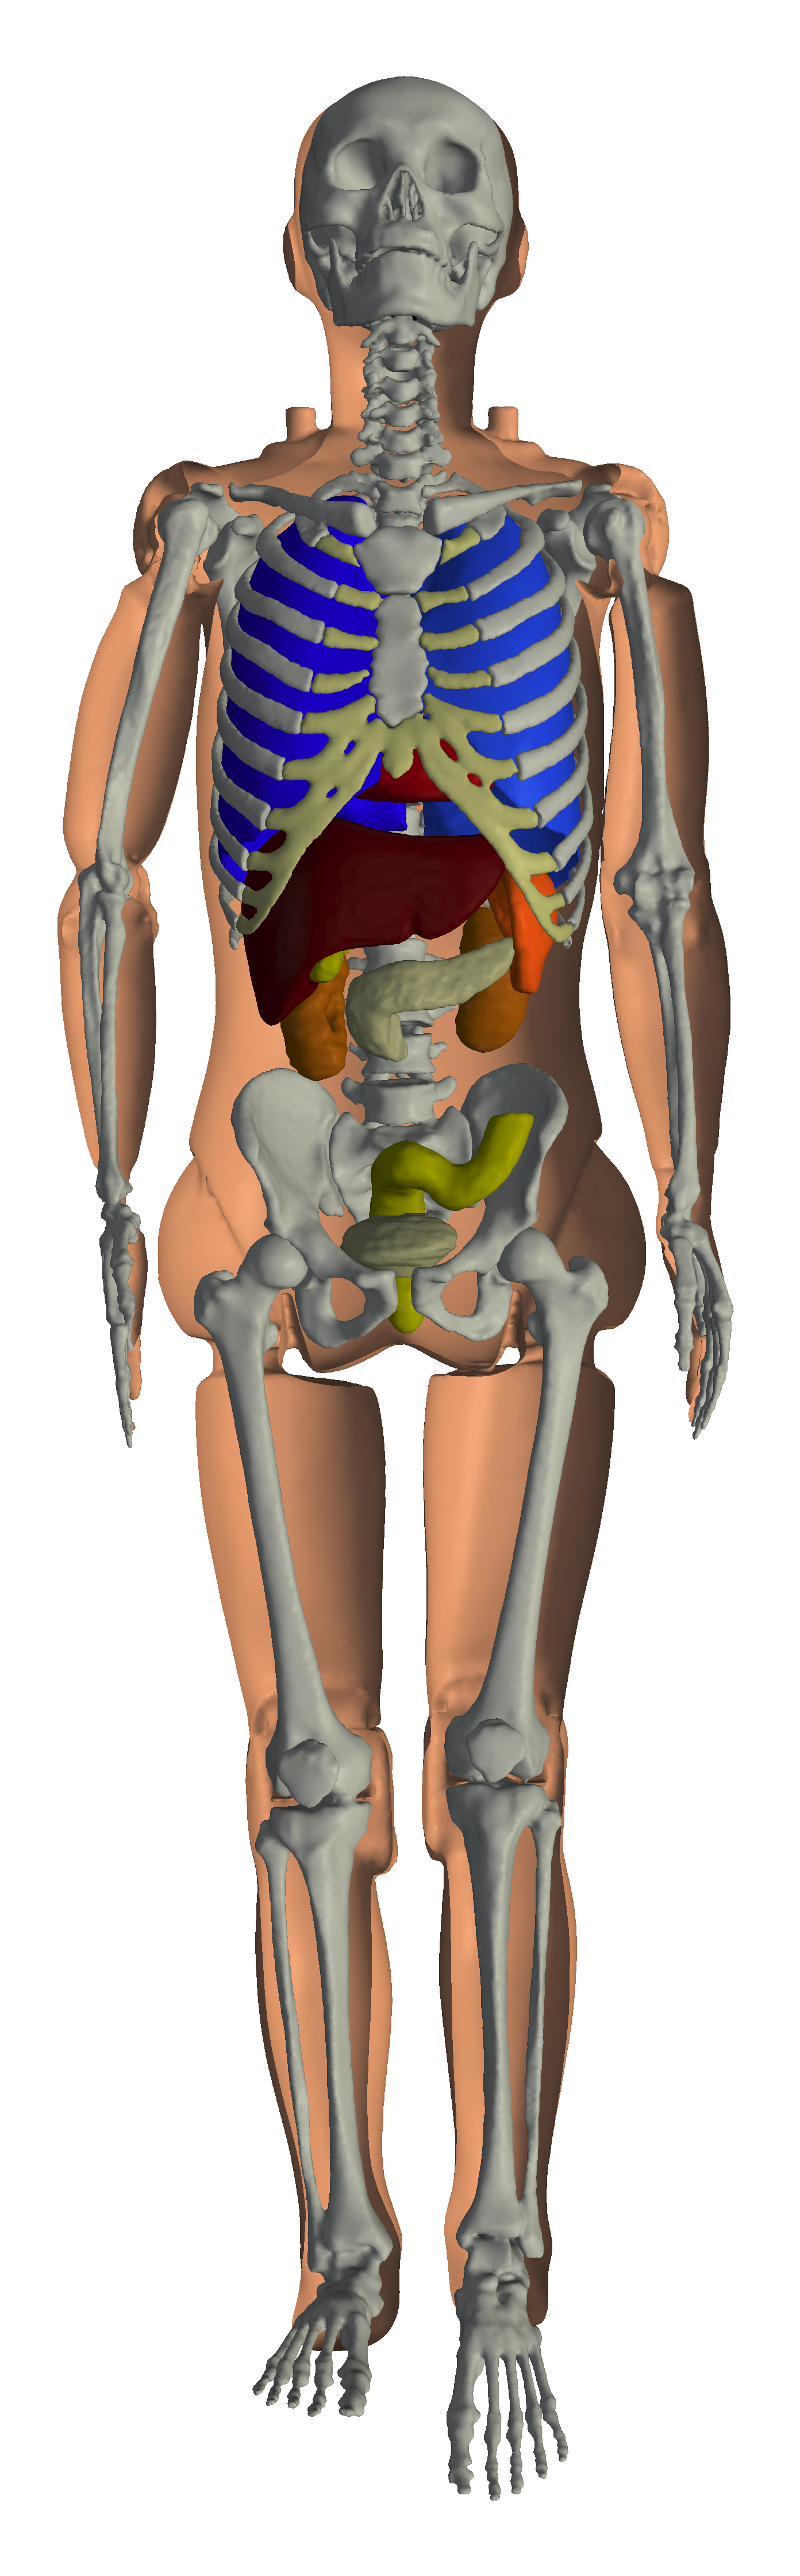
\includegraphics[width=\textwidth,trim={0 1400 0 0},clip]{../img/kyoto}
\end{figure}
\end{columns}
\vfill
\end{frame}
